

%%%%%%%%%%%%%%%%%%%%%%%%%%%%%%%%
%%%%%%%%%%%%%%%%%%%%%%%%%%%%%%%%
\documentclass[12pt]{article}
\usepackage{amsmath, amssymb, amsthm}
\usepackage{graphicx}
\usepackage{float}

\theoremstyle{definition}
\newtheorem*{defn}{Definition}
\newtheorem*{prop}{Proposition}
\newtheorem*{theorem}{Theorem}

%%%%%%%%%%%%%%%%%%%%%%%%%%%%%%%%




%%%%%%%%%%%%%%%%%%%%%%%%%%%%%%%%
%%%%%%%%%%%%%%%%%%%%%%%%%%%%%%%%
\begin{document}

\title{Assignment 3}
\author{Amani Hussien}

\maketitle 

\section{Part 1}%

This program iterates through the recursive function 

 \begin{equation*}
     z_{n+1} = z_n^2+c
 \end{equation*}
over a grid of complex numbers $c=x+iy$ in where $-2<x<2$ and 
$-2<y<2$.
The program tracks each point in the complex plane and determines whether
the sequence is still bounded or has diverged. The following plots are, respectively:


\begin{enumerate}
    \item Bounded vs Diverging plot: an image where points that are bounded are one color and points that have diverged are another.
    \item Divergence iteration plot: a color map showing the iteration number at which each point diverged.
\end{enumerate}

 
\begin{figure}[H]
    \centering
    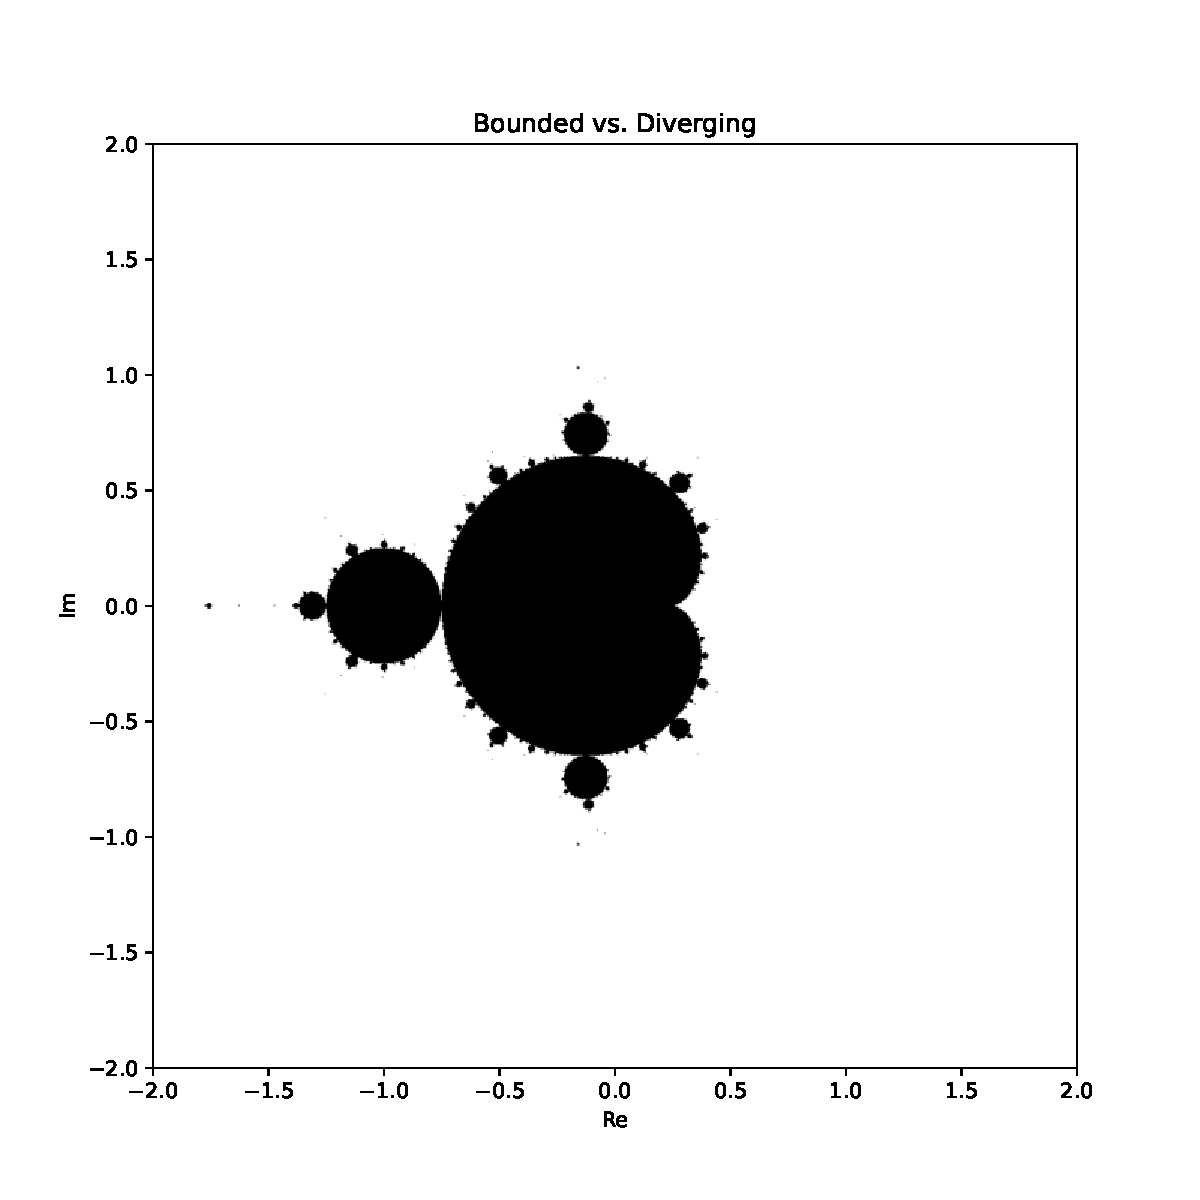
\includegraphics[width=0.6\linewidth]{bounded vs diverging.pdf}

\end{figure}

\begin{figure}[H]
    \centering
    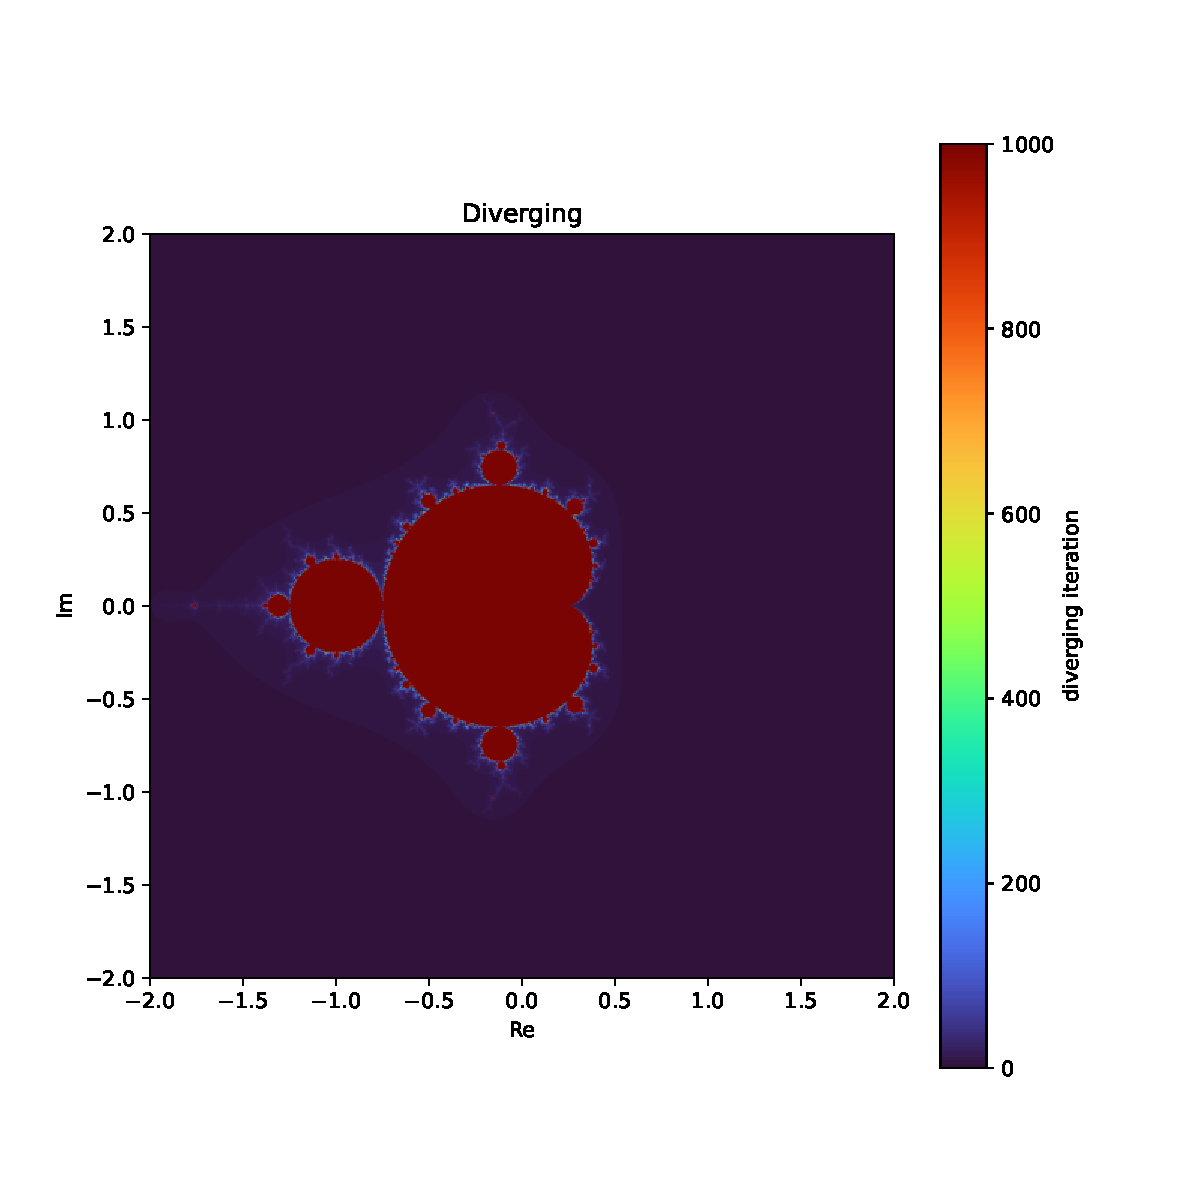
\includegraphics[width=0.6\linewidth]{diverging.pdf}
\end{figure}



\section{Part 2}%

This solves the Lorenz system of differential equations using SciPy's \texttt{solve\_ivp} ODE solver. The Lorenz equations are given by

\[
\frac{dx}{dt} = -\sigma(x-y)
\]

\[
\frac{dy}{dt} = rx-y-xz
\]

\[
\frac{dz}{dt} = -bz+xy
\]

where \(\sigma\) is the Prandtl number, \(r\) is the Rayleigh number, and \(b\) is a dimensionless geometric parameter. The parameters used were

\[
\sigma = 10, \qquad r = 28, \qquad b = \frac{8}{3}
\]

with initial conditions $(x_0,y_0,z_0) = (0,1,0)$

The first figure shows the time-evolution of the y-coordinate over three consecutive time intervals. It is a reproduction of Fig 1. from Lorenz.

\begin{figure}[H]
    \centering
    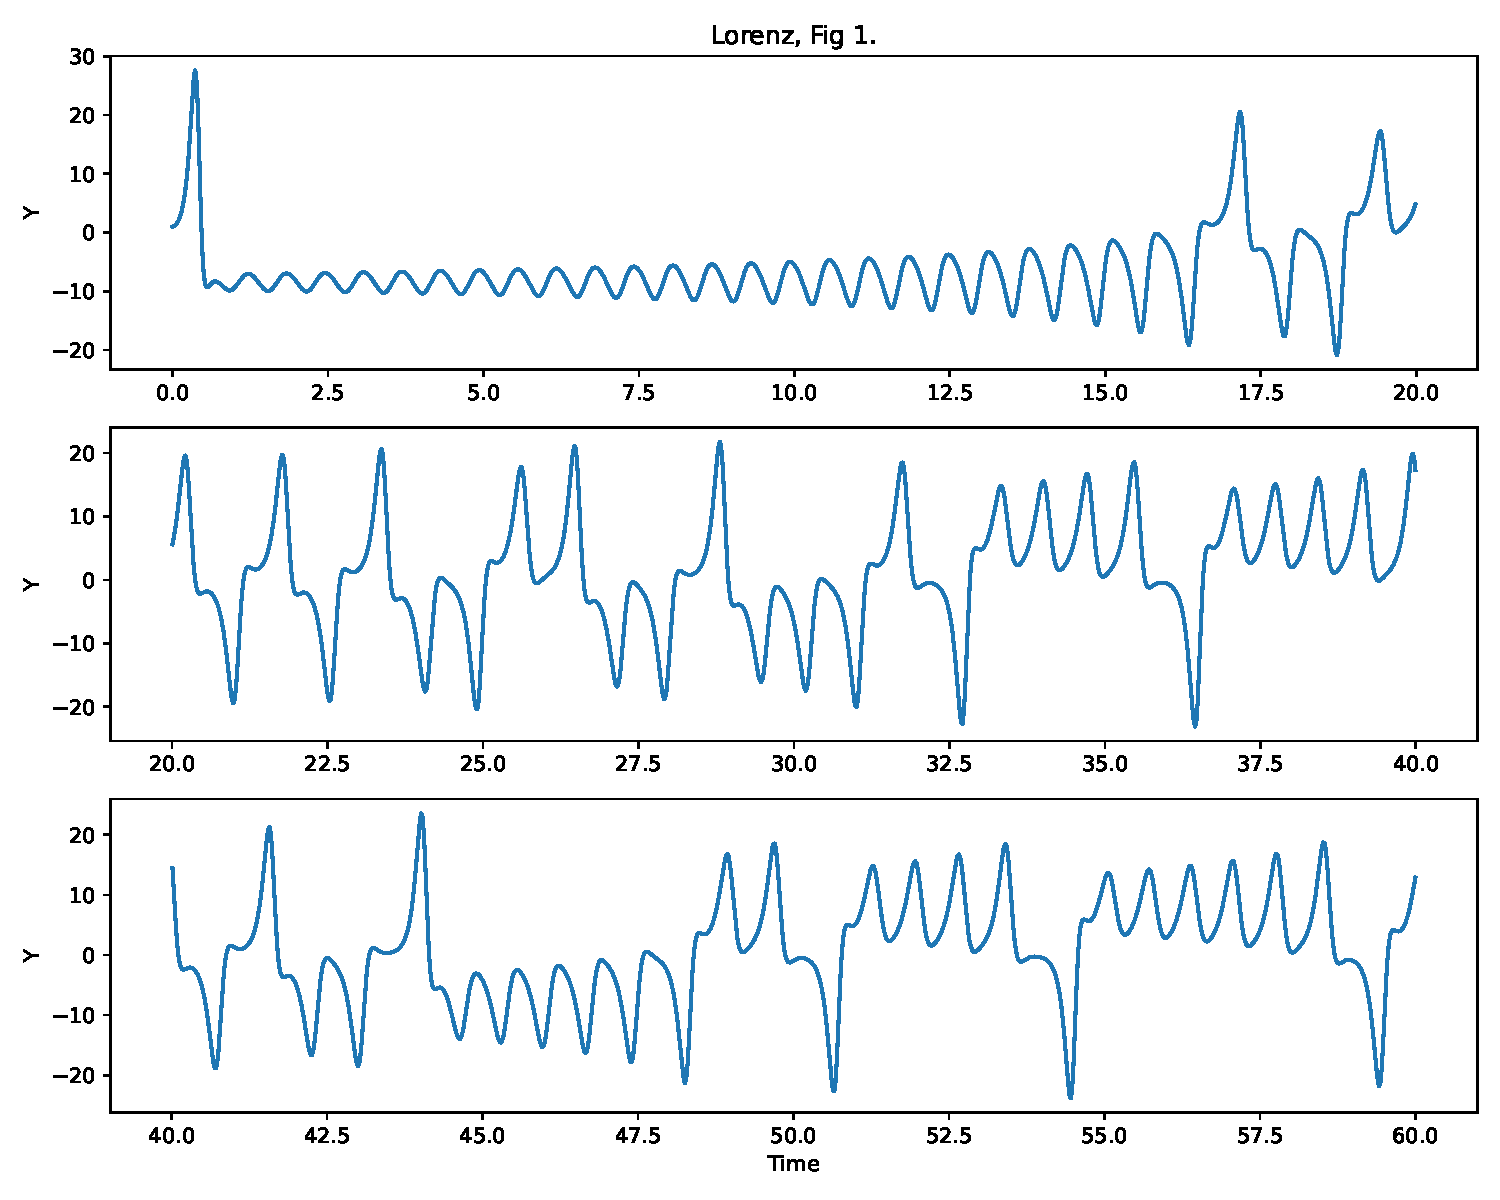
\includegraphics[width=0.7\linewidth]{lorenz1.pdf}
\end{figure}

The second figure shows projections onto the $YZ$ and $XY$ planes. It is a reproduction of Fig 2. from Lorenz.


\begin{figure}[H]
    \centering
    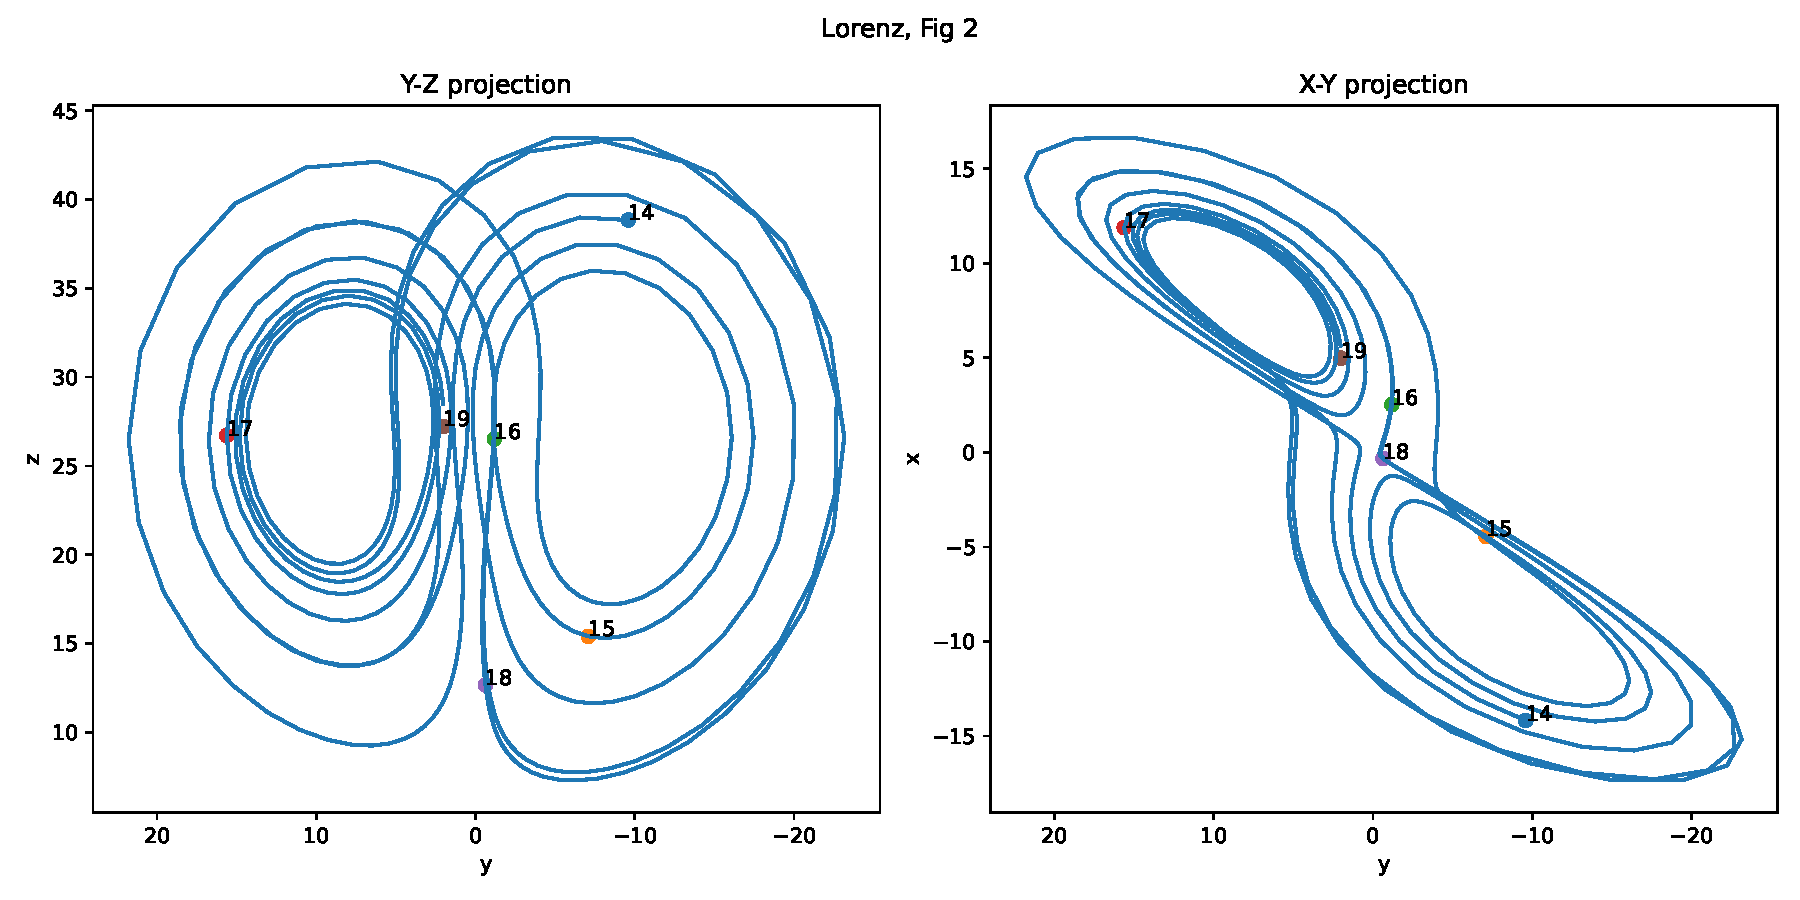
\includegraphics[width=0.8\linewidth]{lorenz2.pdf}
    
\end{figure}

The last figure shows the system solved again with the initial condition differing by \(10^{-8}\) in the \(y\)-component. The distance between these trajectories was then calculated as a function of time.

\begin{figure}[H]
    \centering
    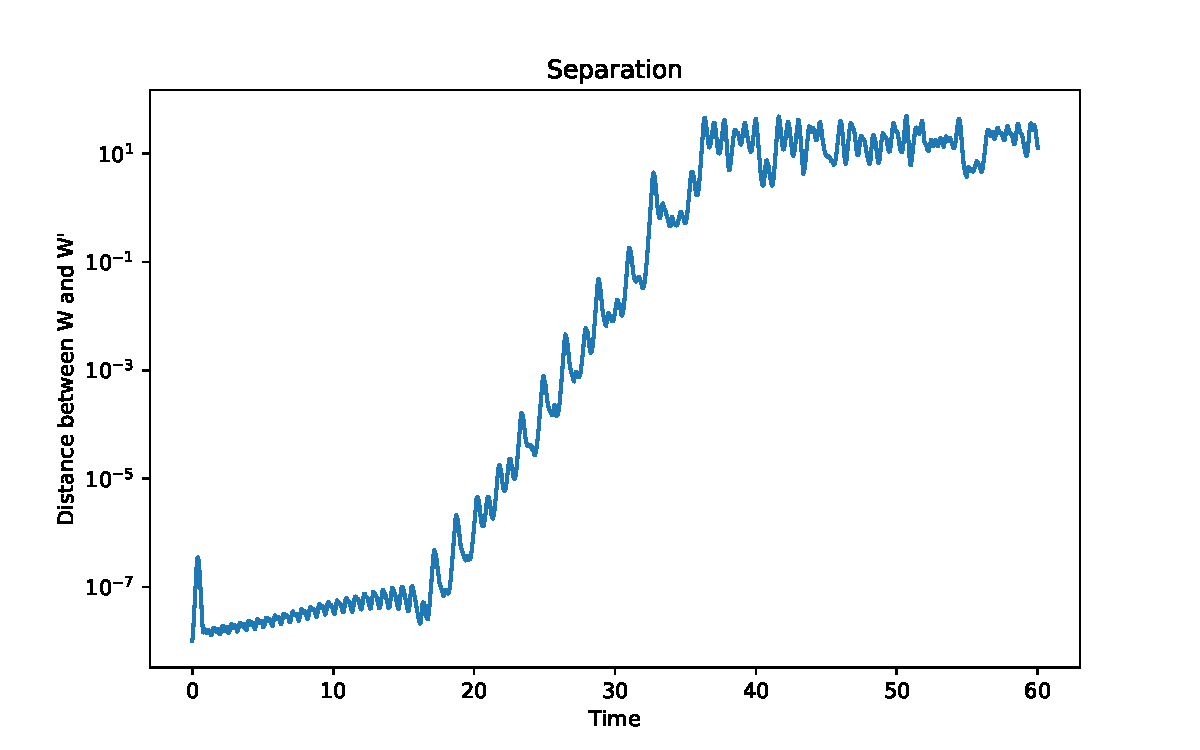
\includegraphics[width=0.7\linewidth]{lorenz3.pdf}
\end{figure}


\end{document}